\documentclass[12pt,a4paper]{article}

% 使用中文宏包
\usepackage[UTF8]{ctex}
\usepackage{graphicx} %插入图片的宏包
\usepackage{float} %设置图片浮动位置的宏包
\usepackage{enumerate}
\usepackage[strings]{underscore}
\usepackage{times}
\usepackage{epsfig}
\usepackage{amsmath}
\usepackage{amssymb}
\usepackage{overpic}
\usepackage{listings}
\usepackage{color}
\usepackage{enumitem}
\setenumerate[1]{itemsep=0pt,partopsep=0pt,parsep=\parskip,topsep=5pt}
\setitemize[1]{itemsep=0pt,partopsep=0pt,parsep=\parskip,topsep=5pt}
\setdescription{itemsep=0pt,partopsep=0pt,parsep=\parskip,topsep=5pt}

\definecolor{mygreen}{rgb}{0,0.6,0}
\definecolor{mygray}{rgb}{0.5,0.5,0.5}
\definecolor{mymauve}{rgb}{0.58,0,0.82}
\lstset{ %
  backgroundcolor=\color{white},   % choose the background color
  basicstyle=\footnotesize,        % size of fonts used for the code
  breaklines=true,                 % automatic line breaking only at whitespace
  captionpos=b,                    % sets the caption-position to bottom
  commentstyle=\color{mygreen},    % comment style
  escapeinside={\%*}{*)},          % if you want to add LaTeX within your code
  keywordstyle=\color{blue},       % keyword style
  stringstyle=\color{mymauve},     % string literal style
}

\usepackage[pagebackref=true,breaklinks=true,letterpaper=true,colorlinks,bookmarks=false]{hyperref}


\def\httilde{\mbox{\tt\raisebox{-.5ex}{\symbol{126}}}}


\graphicspath{{figures/}}

\setcounter{page}{1}

\begin{document}


%%%%%%%%% TITLE

\title{论文阅读笔记:博弈论}
\author{纳文琪}
\maketitle

\section{完全信息静态博弈}
\paragraph{博弈的标准式表述} 包括参与者、每一参与者可供选择的战略集、针对所有参与者可能选择的战略组合和每一个参与者获得的利益,我们用$G={S_1,...,S_n;u_1,...,u_n}$表示博弈。
	\subparagraph{n} 表示参与者的数量, i表示参与者的序号;
	\subparagraph{$S_i$} 表示序号为i的参与者可以选择的战略组合,i的战略空间;
	\subparagraph{$s_i$} 表示战略空间中的一个特定战略;
	\subparagraph{$u_i(s_1,...,s_n)$} 表示i的收益函数,即参与者选择战略$(s_1,...,s_n)$时,第i个参与者的收益。
\subsection{求解方法}	
\paragraph{} 博弈的求解方法包括占优策略均衡、严格下策反复消去法、相对占优策略画线法,这些方法都一定的局限性,并不适合所有的博弈。
\subsubsection{占优策略均衡}
\paragraph{占优策略均衡} 是指这样一种特殊的博弈:某一博弈方的策略可能并不依赖于其他博弈方的策略选择。也就是说,无论所有其他博弈方采取什么策略,该博弈方的“某个策略”始终是最优反应的策略。我们称这种策略为该博弈方的一个“占优策略”(DominantStrategy)或“上策”。
\paragraph{占优策略} 在标准式的博弈G中,令参与者i的两个策略${s_i}',{s_i}'' \in S_i$,如果对其他参与者的每一个可能的战略组合,i选择${s_i}'$的收益都比选择${s_i}''$的收益大,即:$u_i(s_1,...,s_{i-1},{s_i}',s_{i+1},...,s_n) \geq u_i(s_1,...,s_{i-1},{s_i}'',s_{i+1},...,s_n)$,则称${s_i}'$相对于${s_i}''$是占优策略。
由所有博弈中的博弈方的占优策略所组成的策略组合为该博弈的“占优策略均衡” (DominantStrategyEquilibrium)

\subsubsection{严格下策反复消去法}
\paragraph{严格劣战略} 在标准式的博弈G中,令参与者i的两个策略${s_i}',{s_i}'' \in S_i$,如果对其他参与者的每一个可能的战略组合,i选择${s_i}'$的收益比选择${s_i}''$小,即:$u_i(s_1,...,s_{i-1},{s_i}',s_{i+1},...,s_n) < u_i(s_1,...,s_{i-1},{s_i}'',s_{i+1},...,s_n)$,则称${s_i}'$相对于${s_i}''$是严格劣战略。
\paragraph{严格下策反复消去法} 可以归纳如下:首先找出某博弈方的严格劣策略,将它剔除,重新构造一个不包括已剔除策略的新博弈;然后,继续剔除这个新的博弈中某一博弈方的严格劣策略;重复进行这一过程,直到博弈方剩下唯一的策略组合为止。剩下的这个唯一的策略组合,就是这个博弈的均衡解。

\subsubsection{相对占优策略画线法}
\paragraph{} 先找出自己针对其他博弈方每种策略或策略组合的最佳对策,然后在此基础上,通过对其他博弈方策略选择的判断,包括对其他博弈方对自己策略选择的判断等,预测博弈的可能结果和确定自己的最优策略。

\subsection{纳什均衡}

\paragraph{纳什均衡} 在博弈G中,如果战略组合${s_1}^*,...,{s_n}^*$是G的一个纳什均衡,则它要满足:对于每一个参与者i,其战略${s_i}^*$都是他针对其他参与者所选战略的最优反应战略。也就是说,${s_i}^*$是以下优化问题的解:
	\begin{equation}
		\max_{s_i \in S_i} u_i({s_1}^*,...,{s_{i-1}}^*,s_i,{s_{i+1}}^*,...,{s_n}^*)
	\end{equation}
也就是说,在其他参与者的战略可随意变换的情况下,${s_i}^*$使得$u_i$最大。
\paragraph{} 并不是所有的博弈都存在纯策略(PureStrategy)纳什均衡点,但至少存在一个混合策略(MixedStrategy)均衡点

\paragraph{混合战略} 对博弈G和战略$S_i$,参与者i的一个混合战略为概率分布$p_i=(p_{i1},...,p_{iK})$。混合策略的得意函数即是所
\paragraph{纳什定理1} 在一个有n个博弈方的标准博弈G中,如果n是有限的,且$S_i$都是有限集,则该博弈至少存在一个纳什均衡,均衡可能包含混合策略。



\section{完全且完美信息动态博弈}
\paragraph{特点} 这类博弈的特定是:
\begin{itemize}
	\item 行动是顺序发生的
	\item 下一步行动之前,所有以前的行动都可被观察到
	\item 每一可能的行动组合下参与者的收益都是共同知识
\end{itemize}
\paragraph{动态博弈的“扩展型”} 扩展形也称为“博弈树”。动态博弈各个博弈方的选择行为有先后次序,第一个行动选择对应的决策节称为“初始节”,每一个选择节点所包含的所有信息叫做“信息集”。各博弈方的选择行为会依次形成相连的博弈阶段,因此动态博弈中博弈方的一次选择行为常称为一个“阶段”(Stage)。
\begin{figure}[H]
	\centering
	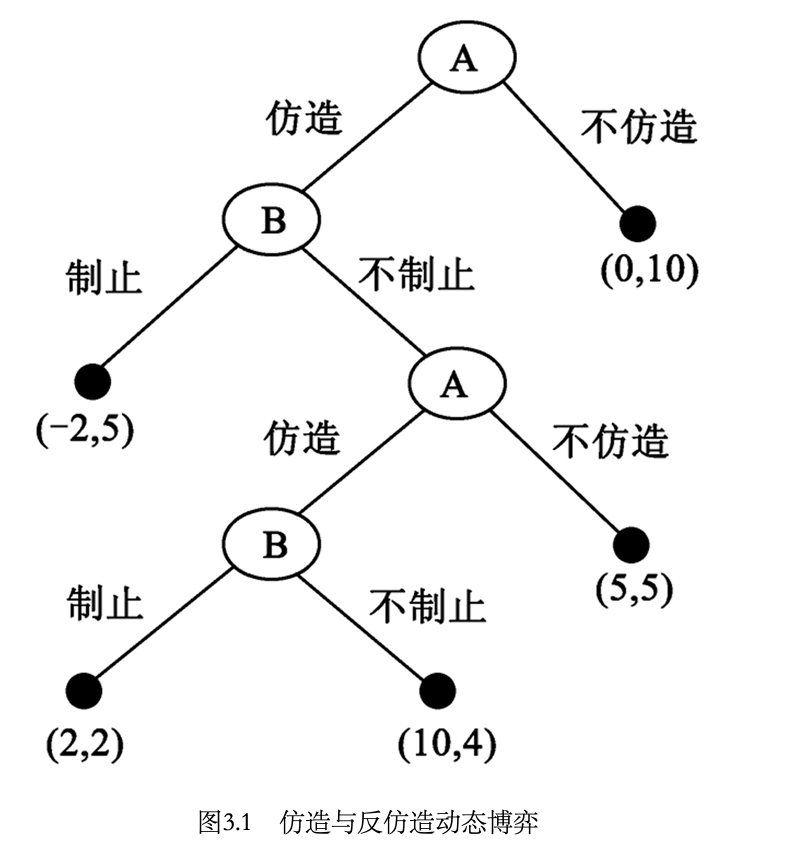
\includegraphics[width=0.6\textwidth]{../images/game-theory-ext-form.png}
	\caption{}
	\label{}
\end{figure}
\subsection{逆向归纳法}
\paragraph{基本思想} 博弈分析从动态博弈的最后一个阶段开始,每一次确定出所分析阶段博弈方的策略选择和路径,然后再确定前一个阶段博弈方的策略选择和路径。

\paragraph{逆向归纳法} 在手雷博弈中,由于由于参与者1的行动$a_1$结束后,参与者2才决定他的行动$a_2$。因此,参与者2面临的决策问题可表示为:
\begin{equation}
	\max_{a_2 \in A_2}u_2(a_1,a_2)
\end{equation}
假定对$A_1$中的每一个动作,参与者2的最优化问题只有唯一的解,用$R_2(a_1)$表示,因此,参与者2的决策问题可以表示为:
\begin{equation}
	\max_{a_2 \in A_2}u_2(a_1,R_2(a_1))
\end{equation}
假定参与者1的最优化问题同样只有一个解,表示为$a_1^*$,则$(a_1^*, R_2(a_1^*))$称为这一博弈的逆向归纳解。
\subsection{子博弈精炼纳什均衡}
\paragraph{子博弈} 由博弈中某一个阶段开始的后续博弈叫做一个“子博弈”(Subgame)
\begin{figure}[H]
	\centering
	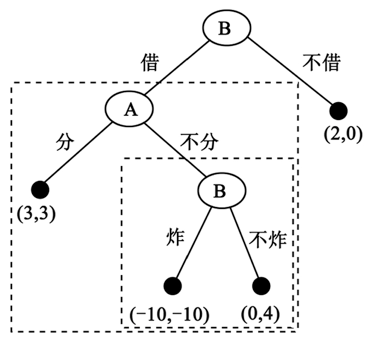
\includegraphics[width=0.6\textwidth]{../images/game-theory-subgame.png}
	\caption{}
	\label{}
\end{figure}
\paragraph{子博弈精炼纳什均衡(Subgame perfectness)} 如果在一个具有完美信息的动态博弈中,各博弈方的策略构成的一个策略组合满足:(1)它是原博弈的纳什均衡;(2)在整个动态博弈及它的所有子博弈中都构成纳什均衡,那么这个策略组合称为该动态博弈的一个“子博弈精练纳什均衡”

\subsection{完全非完美信息两阶段博弈}
\paragraph{特点} 这类博弈与前一类的区别在于,每一阶段都存在着同时行动。
\paragraph{子博弈精炼} 在完全非完美信息两阶段博弈中,参与者1和参与者2同时各自行动,参与者3和参与者4观察第一阶段的结果,再同时各自行动。假定$(a_1^*,a_2^*)$为第一阶段博弈的唯一纳什均衡,则称$(a_1^*,a_2^*,a_3^*(a_1^*,a_2^*),a_4^*(a_1^*,a_2^*))$为博弈的子博弈精炼解。

\subsection{重复博弈}
\paragraph{重复博弈} G(T)表示G进行T次的有效重复博弈,并且在下一次博弈开始前,以前所有的博弈都可被观察到。G(T)的收益为T次博弈收益的简单相加。
\paragraph{定理} 如果G有唯一的纳什均衡,则G(T)有唯一的子博弈精炼解。





\section{不完全信息博弈}
\paragraph{类型} 虽然一些博弈方(如博弈方k)不能确定其他博弈方在一定策略组合下的得益,但一般知道其他博弈方(如博弈方i)的得益有哪些可能的结果,而具体哪种可能的结果会出现则取决于博弈方属于哪种“类型”(Type)。这些“类型”是博弈方自己清楚而其他博弈方无法完全清楚的有关私人内部信息。

\paragraph{静态贝叶斯博弈} 我们用$G=\left \{ A_1, …, A_n; T_1,…,T_n;p_1,…,p_n;u_1,…,u_n \right \} $表示这一博弈。博弈者的行为空间$A_1,…,A_n$,类型空间$T_1,…,T_n$,博弈方的推断$p_1,…,p_n$以及函数$u_1,…,u_n$。博弈者i的类型作为博弈者i的私人信息,决定了博弈i的收益函数$u_i(a_1,…,a_n;t_i)$。博弈者i的推断$p_i(t_{-i}|t_i)$描述了i在给定自己的类型$t_i$时,对其他$n-1$个参与者可能的类型$t_{-i}$的不确定性。


\paragraph{海萨尼转换的基本方法}
\begin{enumerate}
	\item 引进一个虚拟的博弈方“自然”(Nature)或者说“上帝”(God),可称为“博弈方0”,它为每个实际博弈方按随机方式抽取各自的类型,即随机地赋予博弈各方的类型,这些类型构成类型向量$t=(t_1,…,t_n)$,其中$t_i \in T_i, i=1,…,n$;
	\item “自然”只让每个博弈方i知道自己的类型,却不让其他博弈方知道。
	\item 所有的博弈方同时选择行动,即各个实际博弈方同时从各自的行为空间中选择行动方案$a_1,…,a_n$。
	\item 除了博弈方0,即“自然”以外,其余博弈方各自取得得益$u_i=u_i(a_1,…,a_n,t_i)$,其中$i=1,…,n$。
\end{enumerate}
\begin{figure}[H]
	\centering
	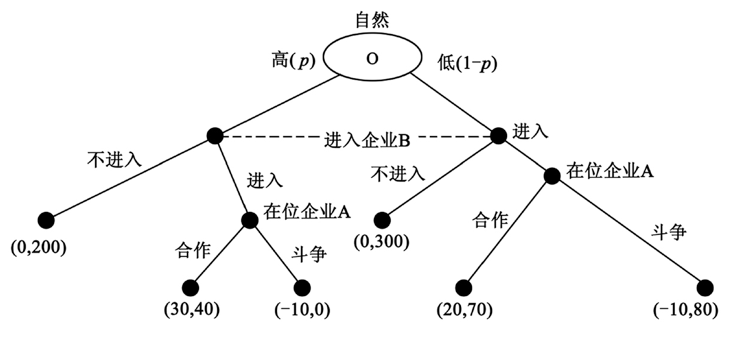
\includegraphics[width=0.8\textwidth]{../images/game-theory-harsany.png}
	\caption{}
	\label{}
\end{figure}

\paragraph{贝叶斯纳什均衡} 在静态贝叶斯博弈G中,如果对任意博弈方i和其每一种可能的类型$t_i$所选择的行动$a_i$都能满足:
\begin{equation}
	\max_{a_i \in A_i} \sum_{t_{-i}} \left \{ u_i [S_1^*(t_1),...,S_{i-1}^*(t_{i-1}),a_i, S_{i+1}^*(t_{i+1}),...,S_n^*(t_n), t_i ]p(t_{-i}|t_i) \right \}
\end{equation}
则称策略组合$S^*=\left \{ (S_1^*,...,S_n^* \right \}$为G的一个纯策略贝叶斯纳什均衡。该定义表明,当静态贝叶斯博弈中博弈方的一个策略组合是贝叶斯纳什均衡时,任何一个博弈方都不想改变自己策略,哪怕只是一种类型下的一个行动,这与纳什均衡的内涵是完全一致的。

\newpage
\section{不完美信息动态博弈}
\paragraph{不完美信息动态博弈的特征}
\begin{itemize}
	\item 动态。各个博弈方的行为有先后次序。
	\item 不完美信息。由于博弈方保密、信息传递不畅或信息的非对称等原因,可能存在后选择的博弈方无法全部了解自己选择之前已经发生的博弈方行动的信息。
	\item 博弈方之间在信息方面的不对称性。
\end{itemize}
\paragraph{示例:旧车市场博弈} 假设旧车有好、差两种方式(type),首先是卖方选择如何使用车子;然后是作为卖方的原车主决定是否卖掉旧车;最后是买方决定是否买下。买方作为一个博弈方对第一阶段卖方行为不了解,即买方具有不完美信息。
\paragraph{不完美信息动态博弈的扩展形} 以上旧车博弈可表示为:
\begin{figure}[H]
	\centering
	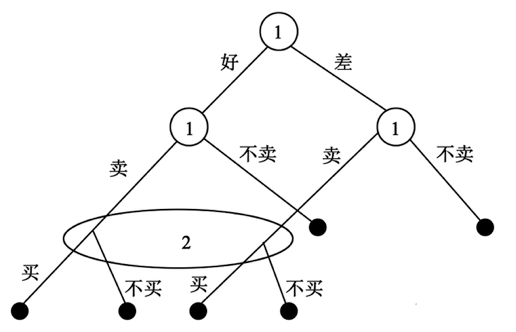
\includegraphics[width=0.8\textwidth]{../images/game-theory-jiuche.png}
	\caption{}
	\label{}
\end{figure}
\subsection{精炼贝叶斯均衡(Perfect Bayesian Equilibrium)}
\paragraph{精炼贝叶斯均衡必须满足的要求}
\begin{enumerate}
	\item 在每一个信息集中,轮到选择的博弈方必须具有一个关于博弈达到该信息集中每个节点可能性的“推断”(Belief)。
	\item 给定各博弈方的“推断”,他们的策略必须是满足“序列理性”的要求
	\item 在均衡路径上的信息集处,“推断”由贝叶斯法则和各博弈方的均衡策略决定。
	\item 对不处于均衡路径上的信息集,“推断”由贝叶斯法则和各博弈方在此处可能有的均衡策略决定。
\end{enumerate}
当一个策略组合及相应的判断满足上面四个要求时,称其为“精练贝叶斯均衡”。

\newpage
\section{不完全信息动态博弈}

\newpage
\section{静态合作博弈}
\paragraph{联盟} 设博弈的局中人集合为N,则对于任意$S \subseteq N$,我们称S为N的一个联盟。我们把S=N称为一个大联盟。
\paragraph{合作博弈的特征型} 给定一个有限的参与人集合N,合作博弈的特征型是有序数对$ <N,v> $,其中特征函数v是从$2^N= \{ S|S \subseteq N\}$到实数集$R^N$的映射,即$<N,v>:2^N \rightarrow R^N,且v(\Phi)=0$。
v的输入和输出都是N维向量,输入表示联盟组合,输出表示各联盟成员的收益(可能是负的)。

\paragraph{支付可转移的联盟型博弈} 是由一个有限的博弈者集合N和一个定义在集合N的函数v所组成的,而这函数v对集合N当中的每一个可能的非空子集S都会进行赋值,其值为一个实数。此类博弈的总收益是可被瓜分(转移)的,因此v的输出是一个总收益。
\paragraph{有结合力的(Cohesive)} 一个支付可以转移的联盟型博弈$<N,v>$是有结合力的,当且仅当,对于集合N的每个分割物(Partition),即$\{S_1,S_2,…,S_m \}$,且,以下的关系式都成立:
\begin{equation}
	v(N) \geq \sum_{j=1}^m v(S_j)
\end{equation}
就是说,如果我们把总联盟N分成m个不相交的小联盟,那么,这m个小联盟的得益的总数是绝不会大于总联盟的得益的。

\paragraph{可加的(Additive)} 在一个支付可转移的联盟型博弈$<N,v>$中,如果对于任意的$S,T \in 2^N, S \cap T = \Phi$有 $v(S)+v(T)\leq v(S \cup T)$,那么,我们称该合作博弈$<N,v>$是超可加的(SupperAdditive)(整体大于部分之和);如果对于任意的$S,T \in 2^N, S \cap T = \Phi$, 有$v(S)+v(T)\geq v(S \cup T)$,那么,我们称该合作博弈$<N,v>$是次可加的(SubAdditive)(整体小于部分之和);如果对于任意的$S,T \in 2^N, S \cap T = \Phi$有$v(S)+v(T)\equiv v(S \cup T)$,那么,我们称该合作博弈是$<N,v>$是可加的。

\paragraph{凸性} $<N,v>$中,若对于任意的$S,T \in 2^N$满足以下条件:
\begin{equation}
	v(S)+v(T) \leq v(S \cup T) + v(S \cap T)
\end{equation}
则称特征函数v具有凸性。
\paragraph{标准化博弈} 若$<N,v>$的特征函数满足下面的两个条件:
\begin{enumerate}
	\item $v(\{i\}) = 0, i = 1,2,...,n$
	\item $v(N) = 1$
\end{enumerate}
则称该博弈为(0,1)标准化博弈。

\subsection{核心和稳定集}
\paragraph{集体理性} 在一个支付可转移的联盟型博弈$<N,v>$中,支付向量$x = (x_1,...x_n)$是符合集体理性的,当且仅当,每位博弈者所分得的支付的总和相等于总联盟的价值,即
\begin{equation}
	x(N) = \sum_{i \in N} x_i = \sum_{i=1}^n x_i = v(N)
\end{equation}

\paragraph{个体理性} 在一个支付可转移的联盟型博弈$<N,v>$中,支付向量$x = (x_1,...x_n)$是符合个体理性的,当且仅当,每位博弈者所分得的支付都比各自为政时高,即$x_i \geq v(\{i\}),i \in N$。

\paragraph{有效分配} 在一个支付可转移的联盟型博弈$<N,v>$中,支付向量$x = (x_1,...x_n)$称为一个分配或有效的分配,当且仅当,它是符合个体理性和集体理性的。

\paragraph{分配集(Imputation)} $<N,v>$的分配集$I(v)$定义为:$I(v) \equiv \{ x \in R^n|x(N)=v(N)\}$, 且对于$\forall i \in N, x_i \geq v(\{i\})$。
\begin{figure}[H]
	\centering
	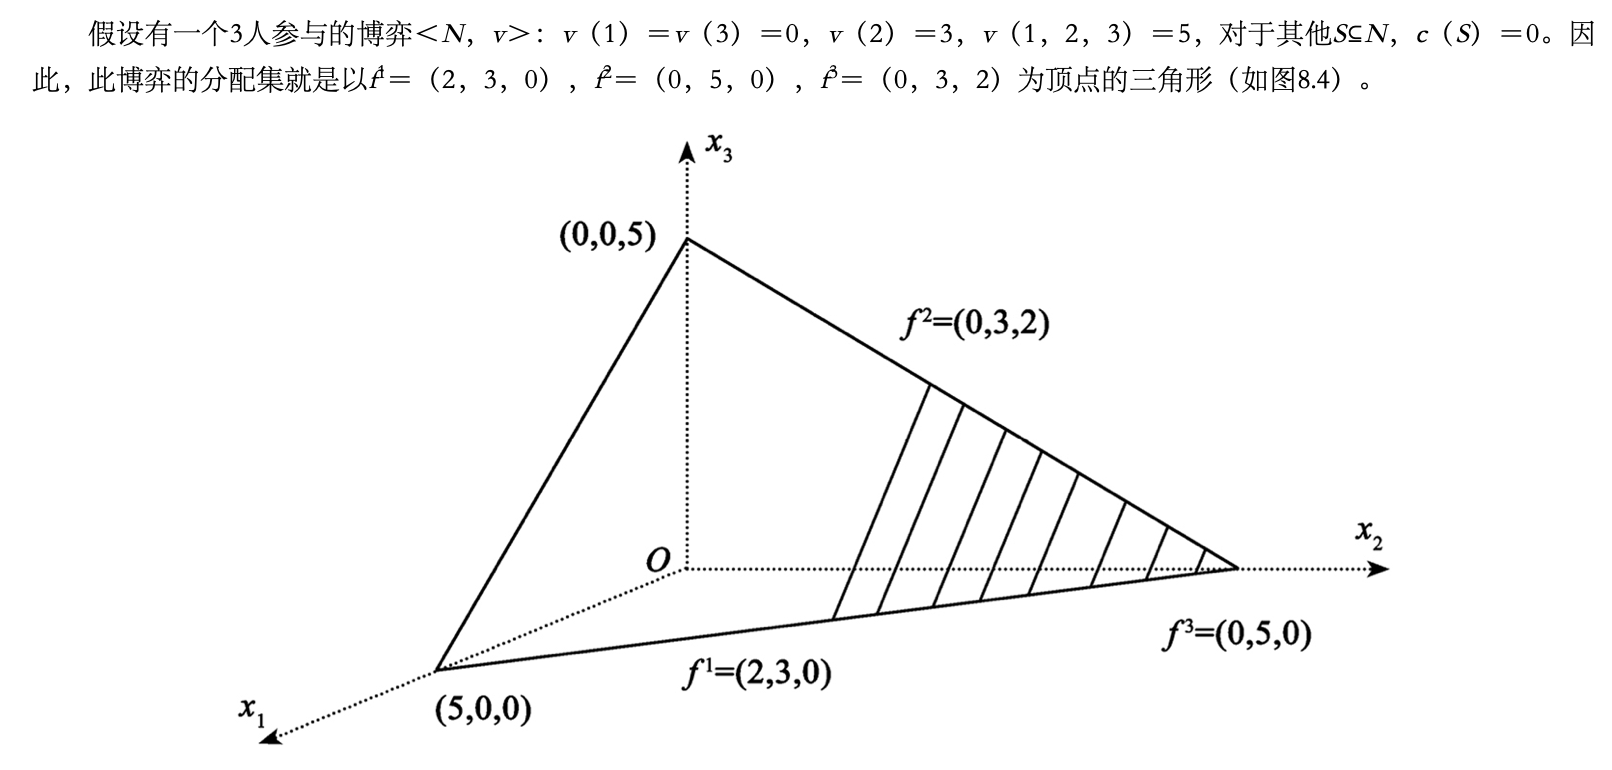
\includegraphics[width=1.0\textwidth]{../images/game-theory-imputation.png}
	\caption{}
	\label{}
\end{figure}

\paragraph{核心} 在一个稳定的分配下,由于组成一个新联盟并不能使该博弈者组合获取更大的得益,任何博弈者组合都不会脱离总联盟,我们把这些稳定的分配的集合称为核心。$<N,v>$的核心$C(v)$是一个集合,当中包含所有能满足以下两个条件的支付向量$x=(x_1,...,x_n)$:
\begin{enumerate}
	\item $x(N)=v(N)$
	\item $x(S) \geq v(S),\forall S \subset N$
\end{enumerate}
核心不仅要满足集体理性,还要满足集合N中每个小联盟S的“理性”。
\begin{figure}[H]
	\centering
	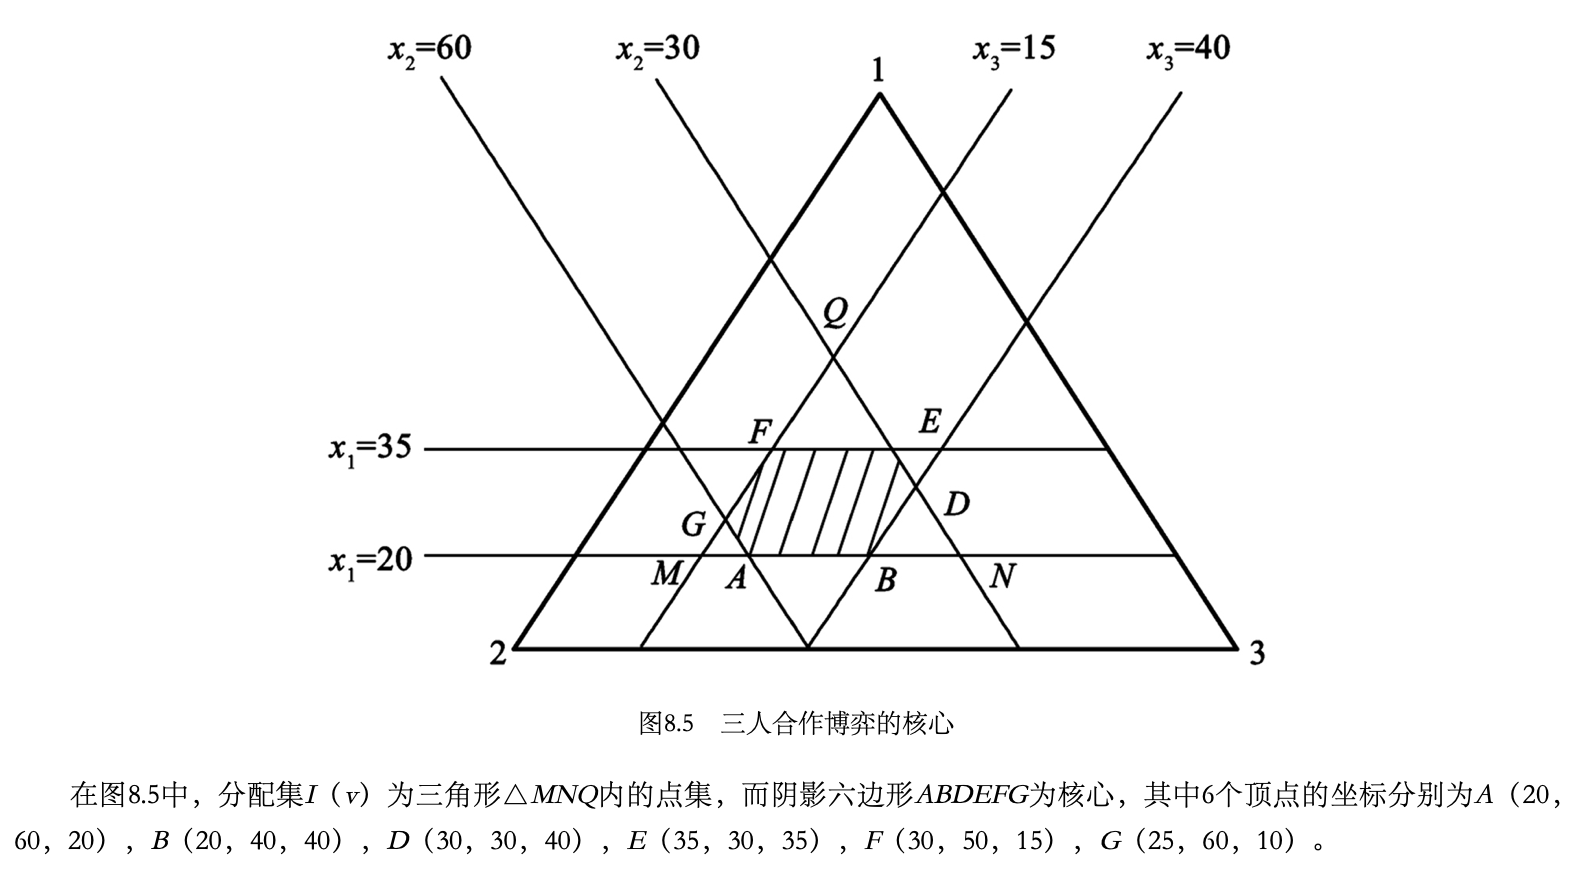
\includegraphics[width=0.8\textwidth]{../images/game-theory-core.png}
	\caption{}
	\label{}
\end{figure}
\paragraph{占优(Dominating)分配} :在一个支付可转移的联盟型合作博弈$<N,v>$中,分配x通过联盟S占优分配y,当且仅当:$x(N)=v(N)$且$x_i \geq v_i, \forall i \in S$,当严格不等式成立时称分配x通过联盟S严格占优于(StrictlyDominate)分配y。

\paragraph{内部稳定性(Internal Stability)} 支付可转移的联盟型合作博弈$<N,v>$的解集符合内部稳定性,如果该集合内的任何分配都不会通过联盟S占优于该集合内的其他分配,也就是说内部稳定性要求联盟内部的任意两个分配不存在占优关系。

\paragraph{外部稳定性(External Stability)} 支付可转移的联盟型合作博弈$<N,v>$的解集符合外部稳定性,如果对于集合外的任意分配,联盟S都存在某配置占优于该集合外的分配。
\paragraph{稳定集(Stable Set)} 在支付可转移的联盟型合作博弈$<N,v>$中,集合X称为稳定集,当且仅当该集合既符合内部稳定性,也符合外部稳定性。
由于合作可能是不稳定的,因此解需要具备的一个重要特性就是稳定性。

\subsection{沙普利值}
\paragraph{载形} 在一个支付可转移的联盟型博弈$<N,v>$中,联盟$N \subseteq U $称为一个载形,当且仅当,对于任何一个联盟$S \subseteq U$,都存在着以下的关系:$v(S)=v(N \cap S)$。一个载形包含了所有会对至少一个联盟作出贡献的博弈者,也就是说,任何不属于载形的博弈者都不会对任何联盟作出贡献。

\paragraph{可互换的} 博弈者i和博弈者j在博弈$<N,v>$中是可互换的,当对于所有包括博弈者i但不包含博弈者j的联盟S,都存在着以下的关系:$v(S \setminus \{i\})\cup\{j\}=v(S)$。也就是说,博弈者i和博弈者j对于联盟S的用处和贡献都是完全一样的。
\paragraph{值} 我们称n维向量$\varphi[v]=(\varphi_1[v],...,\varphi_n[v])$为一个值,这个值包含了n个实数,分别代表着在博弈$<N,v>$中的n位博弈者所分得的支付。

\paragraph{值必须满足的三个公理}
	\subparagraph{效率公理} 如果集合N是一个载形,那么 $\sum_{i \in N}\varphi_i[v] = v(N)$。此公理要求的是集体理性。
	\subparagraph{对称公理}如果博弈者i和博弈者j是可互换的,那么$\varphi_i[v]=\varphi_j[v]$。此公理要求的是博弈者的名称并不会对博弈起任何作用。
	\subparagraph{集成定律}如果$<N,v>$和$<N,u>$是两个博弈,那么$\varphi_i[u+v]=\varphi_i[v]+\varphi_i[u]$。此公理要求的是任何两个独立的博弈联合在一起,那么所组成的新博弈的值是原来的两个博弈的值的直接相加。
\paragraph{沙普利定理} 函数$\varphi$是唯一能够满足以上三个公理的函数,这个函数可以表达为:
\begin{equation}
	\varphi_i[v] = \sum_{S \subseteq N} \gamma_n(S)[v(S)-v(S-\{i\}], \forall i \in N
\end{equation}
其中:
\begin{equation}
	\gamma_n(S) = \frac{(|S|-1)!(n-|S|)!}{n!}
\end{equation}
我们称$\varphi[v]$为沙普利值。
	\subparagraph{$v(S)-v(S-\{i\}$}  表示博弈者i对联盟S的边际贡献;
	\subparagraph{$n!$} 在一个n人博弈中,假定每位博弈者都是随机进入博弈,那么博弈者共有n!种不同的进入博弈的方法;
	\subparagraph{$(|S|-1)!$} 表示博弈者i和S中其他博弈者组成联盟S的可能情况的数量;
	\subparagraph{$(n-|S|)!$} 除了S中的博弈者,其他博弈者可能组成联盟的数量。
	\subparagraph{$\gamma_n(S)$} 是一个有关一位博弈者加入联盟S的特定概率。

根据以上,沙普利值便可理解为每位博弈者在博弈中的每个可能联盟的平均边际贡献率。
\paragraph{沙普利值的三个特征} 个体理性、集体理性、唯一性

\subsection{谈判集、内核及核仁}
\subsubsection{谈判集}
\paragraph{联盟结构} 在一个由n人组成的联盟型博弈中,一个联盟结构就是集合N的一个分割物或一个不相交的子集$T=\{T_1,...,T_n\}$.

\paragraph{特定联盟结构下的分配} 在一个由n人组成的联盟型博弈中,对于联盟结构T,n维支付向量$x=(x_1,...,x_n)$称为一个分配,当且仅当,在每个联盟中,每个成员分得的支付的总和等于该联盟的价值,即:
\begin{equation}
	x_i \geq v({i}) and \sum_{i \in T_k} x_i = v(T_k), k=1,...,n
\end{equation}

\paragraph{异议} 给定博弈者k和l是同属于联盟$T_j$的两位博弈者,那么,博弈者k对l有一个异议$(y,S)$,当且仅当,博弈者k可以提出组成一个包含博弈者k但不包含l的联盟S,然后采用一个S可行的支付向量$y=(y_1,...,y_s)$,从而使得联盟中的每位成员i都获得比现行的支付多。也就是说,博弈者k对l的异议$(y,S)$能满足以下三个条件:
\begin{enumerate}
	\item $S \cap N, k \in S, l \notin S$
	\item $y \in R_s, \sum_{i \in S}y_i = v(S)$
	\item $y_i > x_i, \forall i \in S$
\end{enumerate}

\paragraph{反异议} 对于博弈者k对于l的异议$(y,S)$,博弈者l有一个反异议$(z,Q)$,当且仅当,博弈者l可以提出组成一个包含博弈者l但不包含k的联盟Q,然后采用一个Q可行的支付向量$z=(z_1,...,z_q)$,从而使得联盟Q中属于联盟S的每位成员i的所得都不少于异议$(y,S)$所指定的支付,而联盟Q中不属于联盟S的每位成员i的所得也不会少于现行的支付。也就是说,反异议能满足以下四个条件:
\begin{enumerate}
	\item $Q \cap N, l \in Q, k \notin Q $
	\item $z \in R^q, \sum_{i \in Q} z_i = v(Q) $
	\item $z_i \geq y_i, \forall i \in Q \cap S $
	\item $z_i \geq x_i, \forall i \in Q \setminus S $
\end{enumerate}


\paragraph{谈判集} 在一个支付可转移的n人联盟型博弈$<N,v>$中,对于联盟结构T,谈判集是一个集合,当中包含所有不存在任何具有正当理由的异议的分配$x \in X(T)$,我们用$M_1^i(T)$表示谈判集。

\subsubsection{内核}
\paragraph{过剩} 在一个n人联盟型博弈$<N,v>$中,对于联盟S和分配$x=(x_1,...,x_n)$,在分配x下联盟S的过剩为:
\begin{equation}
	e(S,x)=v(S)-\sum_{i \in S}x_i
\end{equation}
过剩$e(S,x)$表示联盟S的价值与在分配x下联盟S的所有成员的总得益的差,代表着集合S的成员拒绝分配x并组成联盟S的总得益。也就是说,如果过剩$e(S,x)$越大,那么集合S的成员更愿意去组成联盟S。
\paragraph{盈余} 在一个n人联盟型博弈$<N,v>$中,对于分配$x=(x_1,...,x_n)$和两位不同的博弈者i和j,在分配x下博弈者i对j的盈余为$S_{ij}(x)=\max e(S,x), \forall S, i\in S, j\notin S$。i对j的盈余$S_{ij}(x)$就是在博弈者i拒绝与博弈者j合作的情况下,博弈者i所能得到的最好支付。如果盈余$S_{ij}(x)$越大,那么博弈者i与博弈者j合作的愿望就越小。
\paragraph{比重} 在联盟结构为$\tilde{\omega}$的情况下,对于分配x和属于$T_k \in \tilde{\omega}$的两位不同博弈者i和j,博弈者i比j有较大的比重(i Outweighs j),当且仅当$S_{ij}(x)\geq S_{ji}(x)$并且$x_j>v(\{j\})$。我们用$i\succ \succ j$来代表这关系。显然,当$i\succ \succ j$时,由于博弈者i的谈判本钱比博弈者j多,因而分配x便是不稳定的。

\paragraph{内核} 在一个支付可转移的n人联盟型博弈$<N,v>$中,对于联盟结构$\tilde{\omega}$,内核是一个集合,当中包含所有不存在以下关系的分配:
\begin{equation}
	x \in X(\tilde{\omega}), i \succ \succ j, i,j \in T_k, T_k \in \tilde{\omega}
\end{equation}
我们用$X(\tilde{\omega})$来表示联盟性博弈的内核。

\subsubsection{核仁}

\section{动态合作博弈}
\subsection{两人微分合作博弈}

\newpage
\section{演化博弈理论}
\subsection{有限理性与演化博弈理论}
\paragraph{演化博弈理论} 是以有限理性假设为基础,在假定博弈的主体具有有限理性的前提下,分析博弈者的资源配置行为以及对所处的博弈进行策略选择,它分析的是有限理性博弈者的博弈均衡问题。
\paragraph{有限理性} 是指博弈者有一定的统计分析能力和对不同策略下相关得益的事后判断能力,但缺乏事前的预见、预测和判断能力。
\subsection{演化稳定策略}
\paragraph{演化博弈理论的基本模型} 按其所考察的群体数目可分为单群体模型(Monomorphic Population Model)与多群体模型(Polymorphic Populations Model)。按照群体在演化中所受到的影响因素是确定性还是随机性的,演化博弈模型可分为确定性动态模型和随机性动态模型。
\paragraph{演化稳定策略} 如果群体中所有的成员都采取这种策略,那么在自然选择的影响下,将没有突变策略侵犯这个群体。
\newpage
\bibliographystyle{ieeepes}
\bibliography{../Saliency}
\end{document}